\newpage

\colorlet{cluster1}{blue!25}
\colorlet{cluster2}{gray}
\definecolor{cluster3}{rgb}{0.88,1,1}
\begin{table}[h]
    \begin{center}
      \caption{Autovetor - Resultado do conjunto chaves em 3 grupos.}
\begin{tabular}{ |>{\centering\arraybackslash}m{4.9cm} | >{\centering\arraybackslash}m{4.9cm} | >{\centering\arraybackslash}m{4.9cm} | } 
	\hline
	\cellcolor{cluster1}
	\grbox{
   \begin{subfigure}[b]{5cm}
   \centering
   
\includegraphics[width=5cm,height=2cm,keepaspectratio,trim=0 0 0 -5]{images/chaves/0.jpeg}
  \end{subfigure}}{0}
   &
   \cellcolor{cluster1}
   \grbox{
    \begin{subfigure}[b]{5cm}
  \centering
   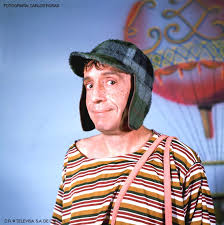
\includegraphics[width=5cm,height=2cm,keepaspectratio,trim=0 0 0 -5]{images/chaves/8.jpeg}
  \end{subfigure}}{8}
   & 
   \cellcolor{cluster1}
   \grbox{
    \begin{subfigure}[b]{5cm}
  \centering
   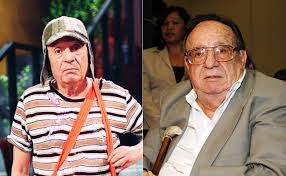
\includegraphics[width=5cm,height=2cm,keepaspectratio,trim=0 0 0 -5]{images/chaves/20.jpeg}
  \end{subfigure}}{20} \\ 
 
 \cellcolor{cluster1}
 \grbox{
   \begin{subfigure}[b]{5cm}
  \centering
   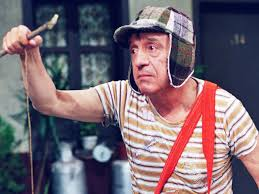
\includegraphics[width=5cm,height=2cm,keepaspectratio,trim=0 0 0 -5]{images/chaves/26.jpeg}
  \end{subfigure}}{26}
   &
   \cellcolor{cluster1}
   \grbox{
   \begin{subfigure}[b]{5cm}
  \centering
   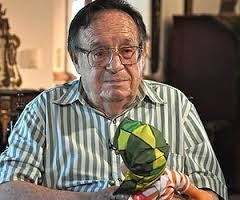
\includegraphics[width=5cm,height=2cm,keepaspectratio,trim=0 0 0 -5]{images/chaves/28.jpeg}
   \end{subfigure}}{28}
   & 
   \cellcolor{cluster1}
   \grbox{
   \begin{subfigure}[b]{5cm}
  \centering
    
\includegraphics[width=5cm,height=2cm,keepaspectratio,trim=0 0 0 -5]{images/chaves/30.jpeg}
  \end{subfigure}}{30} \\ 
   \cellcolor{cluster1}
   \grbox{
   \begin{subfigure}[b]{5cm}
  \centering
   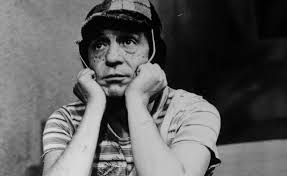
\includegraphics[width=5cm,height=2cm,keepaspectratio,trim=0 0 0 -5]{images/chaves/31.jpeg}
  \end{subfigure}}{\underline{31}}
   &
   \cellcolor{cluster2}
   \grbox{
   \begin{subfigure}[b]{5cm}
  \centering
   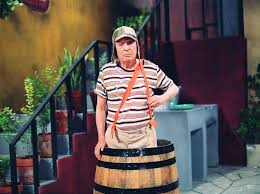
\includegraphics[width=5cm,height=2cm,keepaspectratio,trim=0 0 0 -5]{images/chaves/1.jpeg}
   \end{subfigure}}{1}
   & 
   \cellcolor{cluster2}
   \grbox{
   \begin{subfigure}[b]{5cm}
  \centering
    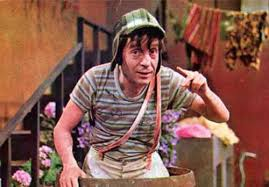
\includegraphics[width=5cm,height=2cm,keepaspectratio,trim=0 0 0 -5]{images/chaves/3.jpeg}
  \end{subfigure}}{3} \\ 
   
   \cellcolor{cluster2}
   \grbox{
   \begin{subfigure}[b]{5cm}
  \centering
   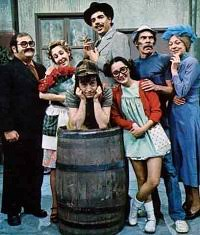
\includegraphics[width=5cm,height=2cm,keepaspectratio,trim=0 0 0 -5]{images/chaves/4.jpeg}
  \end{subfigure}}{4}
   &
   \cellcolor{cluster2}
   \grbox{
   \begin{subfigure}[b]{5cm}
  \centering
   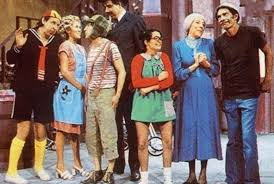
\includegraphics[width=5cm,height=2cm,keepaspectratio,trim=0 0 0 -5]{images/chaves/7.jpeg}
   \end{subfigure}}{7}
   & 
   \cellcolor{cluster2}
   \grbox{
   \begin{subfigure}[b]{5cm}
  \centering
    
\includegraphics[width=5cm,height=2cm,keepaspectratio,trim=0 0 0 -5]{images/chaves/9.jpeg}
  \end{subfigure}}{9} \\ 
   
   \cellcolor{cluster2}
   \grbox{
   \begin{subfigure}[b]{5cm}
  \centering
   
\includegraphics[width=5cm,height=2cm,keepaspectratio,trim=0 0 0 -5]{images/chaves/10.jpeg}
  \end{subfigure}}{10}
   &
   \cellcolor{cluster2}
   \grbox{
   \begin{subfigure}[b]{5cm}
  \centering
   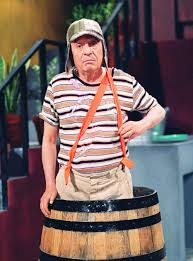
\includegraphics[width=5cm,height=2cm,keepaspectratio,trim=0 0 0 -5]{images/chaves/11.jpeg}
   \end{subfigure}}{11}
   & 
   \cellcolor{cluster2}
   \grbox{
   \begin{subfigure}[b]{5cm}
  \centering
    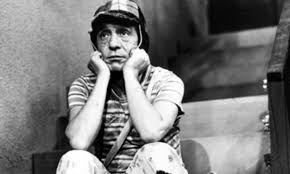
\includegraphics[width=5cm,height=2cm,keepaspectratio,trim=0 0 0 -5]{images/chaves/12.jpeg}
  \end{subfigure}}{12} \\ 
   
   \cellcolor{cluster2}
   \grbox{
   \begin{subfigure}[b]{5cm}
  \centering
   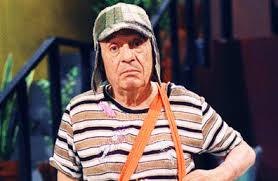
\includegraphics[width=5cm,height=2cm,keepaspectratio,trim=0 0 0 -5]{images/chaves/13.jpeg}
  \end{subfigure}}{13}
   &
   \cellcolor{cluster2}
   \grbox{
   \begin{subfigure}[b]{5cm}
  \centering
   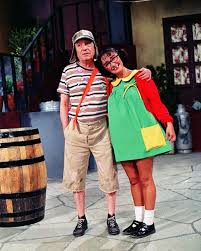
\includegraphics[width=5cm,height=2cm,keepaspectratio,trim=0 0 0 -5]{images/chaves/15.jpeg}
   \end{subfigure}}{15}
   & 
   \cellcolor{cluster2}
   \grbox{
   \begin{subfigure}[b]{5cm}
  \centering
    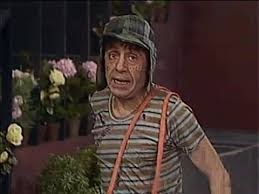
\includegraphics[width=5cm,height=2cm,keepaspectratio,trim=0 0 0 -5]{images/chaves/18.jpeg}
  \end{subfigure}}{\underline{18}} \\ 
   
   \cellcolor{cluster2}
   \grbox{
   \begin{subfigure}[b]{5cm}
  \centering
   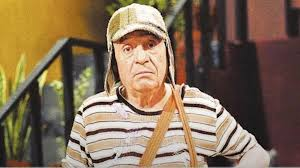
\includegraphics[width=5cm,height=2cm,keepaspectratio,trim=0 0 0 -5]{images/chaves/21.jpeg}
  \end{subfigure}}{21}
   &
   \cellcolor{cluster2}
   \grbox{
   \begin{subfigure}[b]{5cm}
  \centering
   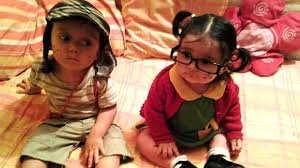
\includegraphics[width=5cm,height=2cm,keepaspectratio,trim=0 0 0 -5]{images/chaves/22.jpeg}
   \end{subfigure}}{22}
   & 
   \cellcolor{cluster2}
   \grbox{
   \begin{subfigure}[b]{5cm}
  \centering
    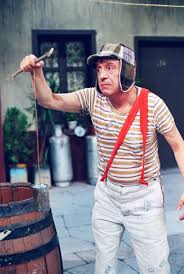
\includegraphics[width=5cm,height=2cm,keepaspectratio,trim=0 0 0 -5]{images/chaves/23.jpeg}
  \end{subfigure}}{23} \\ 
   
   \cellcolor{cluster2}
   \grbox{
   \begin{subfigure}[b]{5cm}
  \centering
   
\includegraphics[width=5cm,height=2cm,keepaspectratio,trim=0 0 0 -5]{images/chaves/24.jpeg}
  \end{subfigure}}{24}
   &
   \cellcolor{cluster2}
   \grbox{
   \begin{subfigure}[b]{5cm}
  \centering
   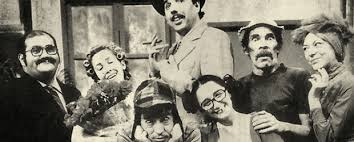
\includegraphics[width=4.2cm,height=2cm,keepaspectratio,trim=0 0 0 -5]{images/chaves/25.jpeg}
   \end{subfigure}}{25}
   & 
   \cellcolor{cluster2}
   \grbox{
   \begin{subfigure}[b]{5cm}
  \centering
    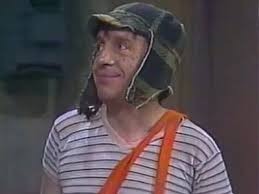
\includegraphics[width=5cm,height=2cm,keepaspectratio,trim=0 0 0 -5]{images/chaves/27.jpeg}
  \end{subfigure}}{28} \\
 
 \cellcolor{cluster2}
 \grbox{
 \begin{subfigure}[b]{5cm}
  \centering
   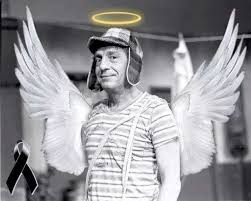
\includegraphics[width=5cm,height=2cm,keepaspectratio,trim=0 0 0 -5]{images/chaves/29.jpeg}
  \end{subfigure}}{29}
   &
   \cellcolor{cluster3}
   \grbox{
   \begin{subfigure}[b]{5cm}
  \centering
   
\includegraphics[width=5cm,height=2cm,keepaspectratio,trim=0 0 0 -5]{images/chaves/2.jpeg}
   \end{subfigure}}{2}
   & 
   \cellcolor{cluster3}
   \grbox{
   \begin{subfigure}[b]{5cm}
  \centering
    
\includegraphics[width=5cm,height=2cm,keepaspectratio,trim=0 0 0 -5]{images/chaves/5.jpeg}
  \end{subfigure}}{5} \\
  \cellcolor{cluster3}
  \grbox{
 \begin{subfigure}[b]{5cm}
  \centering
   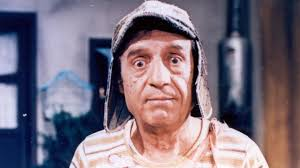
\includegraphics[width=5cm,height=2cm,keepaspectratio,trim=0 0 0 -5]{images/chaves/6.jpeg}
  \end{subfigure}}{6}
   &
   \cellcolor{cluster3}
   \grbox{
   \begin{subfigure}[b]{5cm}
  \centering
   
\includegraphics[width=5cm,height=2cm,keepaspectratio,trim=0 0 0 -5]{images/chaves/14.jpeg}
   \end{subfigure}}{14}
   & 
   \cellcolor{cluster3}
   \grbox{
   \begin{subfigure}[b]{5cm}
  \centering
    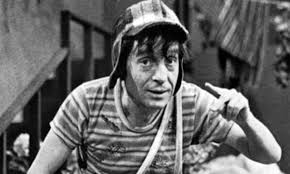
\includegraphics[width=5cm,height=2cm,keepaspectratio,trim=0 0 0 -5]{images/chaves/16.jpeg}
  \end{subfigure}}{16} \\
 \cellcolor{cluster3}
 \grbox{
 \begin{subfigure}[b]{5cm}
  \centering
   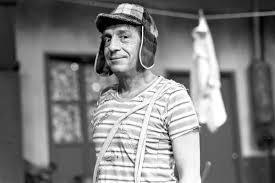
\includegraphics[width=5cm,height=2cm,keepaspectratio,trim=0 0 0 -5]{images/chaves/17.jpeg}
  \end{subfigure}}{17}
   &
   \cellcolor{cluster3}
   \grbox{
   \begin{subfigure}[b]{5cm}
  \centering
   
\includegraphics[width=5cm,height=2cm,keepaspectratio,trim=0 0 0 -5]{images/chaves/19.jpeg}
  \end{subfigure}}{\underline{19}}
   &
   \cellcolor{cluster3}
   \grbox{
   \begin{subfigure}[b]{5cm}
  \centering
   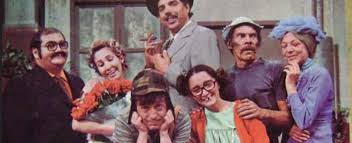
\includegraphics[width=4.2cm,height=2cm,keepaspectratio,trim=0 0 0 -5]{images/chaves/32.jpeg}
  \end{subfigure}}{32}  \\
  \hline
\end{tabular}
\label{chavesAutoVetor}
\legend{\textbf{Fonte:} \citeonline{google2}.}
\end{center}
\end{table}